\subsection{Three scientific case studies}
\label{sec:cases}

% Added 10 September 2026 after the Terminus-2 runs on the three cases.
% FEDOT.LLM rows and paragraph are filled in once cases_fedot.sh has run.

Benchmarks measure what they were built to measure. To see the same design on
tasks that exist because someone needed the answer, we took three published
studies with an author-reported baseline and made each a Harbor task.
Figure~\ref{fig:cases} shows what they ask. Maize grain yield in the
Genomes-to-Fields trials~\citep{kick2023yield} is predicted for location-years
the model has never seen, from pedigree, site and management columns, with the
authors' own split of $158$ location-years. Exit state of jobs on the Fugaku
supercomputer~\citep{antici2025fdata} is predicted from what the scheduler
knows at submission time, so that a job likely to fail can be flagged before
it runs; the classes are imbalanced and a constant predictor already scores
$\caseFdataFloor$. Glass-transition temperature of polymers in
OpenPoly~\citep{wang2025openpoly} is predicted from a PSMILES string, so the
agent must decide how a repeat unit becomes numbers before any model is fit.

\begin{figure*}[t]
\centering
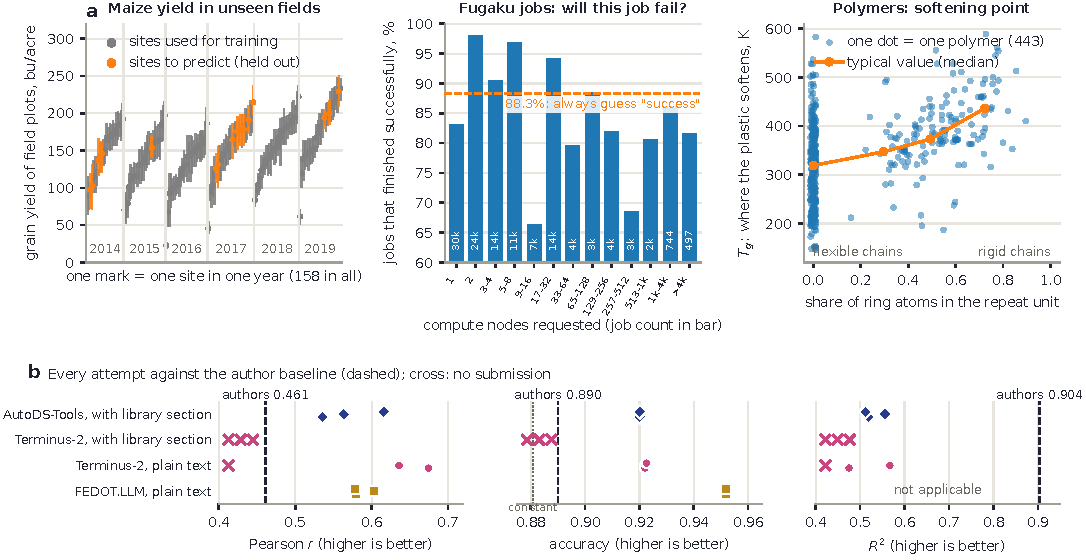
\includegraphics[width=0.78\textwidth]{figures/fig_cases.pdf}
\caption{What the three case studies ask, drawn from the open source data.
Left: each mark is one field site in one year, the dot its median plot yield
and the bar the middle half of its plots; the orange sites are held out, so
the model must predict yield where it has seen no plot at all. Middle: jobs on
the Fugaku supercomputer grouped by the number of compute nodes requested,
with the share that finished successfully; a model that always predicts
success is right $88.3\%$ of the time, and a useful one must beat that from
what is known when the job is submitted. Right: each dot is a polymer, its
softening temperature $T_g$ against how much of its repeat unit is made of
rigid rings; the model must recover this trend from the structure string
alone.}
\label{fig:cases}
\end{figure*}

Each task text was written for the AutoDS-Tools runs of July 2026 and sits at the far
end of the prescription axis of Section~\ref{sec:axis}: it names LightAutoML~\citep{vakhrushev2021lightautoml}
as the required library, supplies a working snippet, lists the columns that
leak the target, describes the split and states the author baseline as the
number to beat. We ran Terminus-2 on that text and on the same text with the
library section removed, three attempts each, on the machine and at the
concurrency of Section~\ref{sec:mlab}, with data, image and scorer shared
between the two texts. AutoDS-Tools enters with its single July run per case.
FEDOT.LLM enters on the two tabular cases with the plain text, three attempts
each and a $40$-minute backend budget (Section~\ref{sec:deviations}); its tool
choice is welded in, so the library section is no condition for it, and a
check run with it in place returned the same F-DATA scores.
Two of the three splits are proxies. F-DATA is one month of logs (April 2021)
with a random $80/20$ split on request-time attributes, so the author figure is
a reference from a different split. OpenPoly is a random $80/20$ split of the
$443$ literature polymers with a measured $T_g$, an $89$-row test set, where
the authors used their full dataset. Table~\ref{tab:cases} gives every row.

\begin{table*}[t]
\centering
\caption{Three scientific case studies, one row per system and task text: the published text with its library section, or the same text without it (plain). $n$ counts attempts that left a submission; mean, min and max are over those; minutes are the median agent time per attempt. Bold: the best system mean per case.}
\label{tab:cases}
\small
\setlength{\tabcolsep}{5pt}
\begin{tabular}{llllcrrrr}
\toprule
Case & Metric & System & Text & $n$ & mean & min & max & min/attempt \\
\midrule
Maize yield (G2F) & Pearson $r$ $\uparrow$ & \emph{authors} & & & 0.461 & & & \\
 & & AutoDS-Tools & with library section & 3/3 & 0.572 & 0.536 & 0.616 & 14.1 \\
 & & Terminus-2 & plain & 2/3 & \textbf{0.655} & 0.636 & 0.674 & 2.1 \\
 & & Terminus-2 & with library section & 0/3 & -- & -- & -- & 4.0 \\
 & & FEDOT.LLM & plain (library built in) & 3/3 & 0.587 & 0.578 & 0.603 & 52.8 \\
\midrule
Fugaku exit state (F-DATA) & Accuracy $\uparrow$ & \emph{authors} & & & 0.890 & & & \\
 & & AutoDS-Tools & with library section & 3/3 & 0.920 & 0.920 & 0.920 & 20.1 \\
 & & Terminus-2 & plain & 3/3 & 0.922 & 0.922 & 0.923 & 1.1 \\
 & & Terminus-2 & with library section & 0/3 & -- & -- & -- & 2.5 \\
 & & FEDOT.LLM & plain (library built in) & 3/3 & \textbf{0.952} & 0.952 & 0.952 & 45.4 \\
\midrule
Polymer $T_g$ (OpenPoly) & $R^2$ $\uparrow$ & \emph{authors} & & & 0.904 & & & \\
 & & AutoDS-Tools & with library section & 3/3 & \textbf{0.529} & 0.512 & 0.556 & 13.1 \\
 & & Terminus-2 & plain & 2/3 & 0.521 & 0.475 & 0.567 & 3.2 \\
 & & Terminus-2 & with library section & 0/3 & -- & -- & -- & 2.6 \\
\bottomrule
\end{tabular}
\begin{tablenotes}\footnotesize
\item AutoDS-Tools rows run the published text with the system's own instruction file off. FEDOT.LLM cannot act on the library section and has no molecular featurisation, so it has one row and was not run on OpenPoly. F-DATA: majority class scores 0.881. OpenPoly: the author figure is on the full dataset, ours on a subset with an 89-row test split, so that row is indicative only.
\end{tablenotes}
\end{table*}


Unaided, Terminus-2 matched or exceeded the author baselines on both tasks
with a comparable split. On maize its two scoring attempts reached Pearson
$r$ of $\caseTermPlainMaizeMin$ and $\caseTermPlainMaizeMax$ against the
authors' best model at $\caseAuthorMaize$, and normalised RMSE of
$\caseTermPlainMaizeNormRmse$ on average against the authors' $0.948$; the
July AutoDS-Tools run had beaten the authors on $r$
($\caseAutoDSMaizeMean$) while losing on error ($\caseAutoDSMaizeNormRmse$),
and Terminus-2 wins on both. On F-DATA all three attempts scored
$\caseTermPlainFdataMean$ accuracy against the authors' $\caseAuthorFdata$,
with balanced accuracy $\caseTermPlainFdataBalancedAccuracy$, level with the
July run. On OpenPoly it reached $R^2$ of $\caseTermPlainPolyMin$ and
$\caseTermPlainPolyMax$, around the July run's $\caseAutoDSPolyMean$ and far
from the authors' full-data $\caseAuthorPoly$, a row we do not interpret. The
traces show what it reached for: on F-DATA a random forest or XGBoost with
class weights, on maize gradient boosting over label-encoded pedigree and site
columns, on OpenPoly RDKit~\citep{rdkit} fingerprints and descriptors under
XGBoost, the published recipe, arrived at without being told.

The prescription cost Terminus-2 every trial. With the library section in the
text, \caseTermPrescLost{} of \caseTermPrescTotal{} attempts ended without a
submission; without it, \caseTermPlainLost{} of \caseTermPlainTotal{}. Every
lost trial ends as in Section~\ref{sec:kdiscterm}: a fit still running in the
foreground and an agent that declared the task complete after $1.5$ to $5.5$
minutes. The prescribed call, LightAutoML at its defaults, takes
$\caseLamaFitFdataMin$ minutes on the F-DATA table and $\caseLamaFitMaizeMin$
on the maize table, and the prescribed RDKit snippet prints a warning per
molecule, so every prescribed attempt outlived the agent's patience; unaided,
the agent chose estimators that return in seconds. AutoDS-Tools finished the
same text in July 2026, its repair loop absorbing the wait. The same text
therefore helps AutoDS-Tools and loses every Terminus-2 attempt where
LightAutoML is a sound choice, repeating Section~\ref{sec:kdiscterm}.

The rigid pipeline is the best system on one of the two tables it can read.
On F-DATA, FEDOT.LLM reached $\caseFedotPlainFdataMean$ accuracy in all three
attempts, with balanced accuracy $\caseFedotPlainFdataBalancedAccuracy$
against $\caseTermPlainFdataBalancedAccuracy$ for Terminus-2 and
$\caseAutoDSFdataBalancedAccuracy$ for AutoDS-Tools: the budget it spends on
tuning a fixed backend buys three points of accuracy and fourteen of balanced
accuracy over two agents that fit one model and stop. On maize it sits between
them, Pearson $r$ of $\caseFedotPlainMaizeMin$ to $\caseFedotPlainMaizeMax$
against $\caseTermPlainMaizeMin$ to $\caseTermPlainMaizeMax$ for Terminus-2
and $\caseAutoDSMaizeMean$ for AutoDS-Tools, and its normalised RMSE of
$\caseFedotPlainMaizeNormRmse$ beats the authors' $0.948$. Its attempts took
$\caseFedotPlainMaizeMinutes$ minutes of the hour on the larger table, because
the backend treats its budget as advice.

\paragraph{Observation 8} On three published tasks Terminus-2 with the open 31B
model and the plain task text matched or beat the author baselines where the split is comparable, and on
OpenPoly it rediscovered the published featurisation. The library prescription
that AutoDS-Tools ran on in July 2026 cost Terminus-2 all \caseTermPrescTotal{}
attempts. FEDOT.LLM, which cannot use the prescription, beat both agents on
F-DATA, where tuning a fixed backend is the whole task.
